\section{Comparison of encodings}\label{sec:encodings}

This section compares eight encodings under identical physical conditions: the same simulator, the same device-parameter and
optical-power ranges, the same readout (31 lines, 8 taps), the same noise model, and the same number of random operating points
with the same selection procedure (Section~\ref{sec:protocol}). Table~\ref{tab:encodings} summarises the three tasks with and
without noise, and Fig.~\ref{fig:encodings} plots the same numbers.

% generated by experiments/make_table1.py; do not edit by hand
\begin{table*}[htbp]
\centering
\caption{Test error (NMSE, lower is better) of each encoding and the baselines. Each encoding draws 256 random operating points over the same ranges; the point is chosen on the mean validation error of new runs and the mean test error over six further pairs of new runs is reported, as the geometric mean over three series; the readout is trained on one run and tested on another with independent noise. The best resonator encoding in each column is in bold. The ESN has the same readout dimension as the resonator (31 nodes, the same delay taps) and uses a single random reservoir; under realistic noise its input noise is $3\times10^{-3}$; stronger software baselines are in Section~\ref{sec:software}. Channel equalisation under realistic noise uses test parts of 5000 symbols.}
\label{tab:encodings}
\footnotesize\setlength{\tabcolsep}{4pt}
\begin{tabular}{lcccccc}
\toprule
 & \multicolumn{2}{c}{Mackey--Glass (10 steps)} & \multicolumn{2}{c}{channel equalisation} & \multicolumn{2}{c}{NARMA-10} \\
\cmidrule(lr){2-3}\cmidrule(lr){4-5}\cmidrule(lr){6-7}
encoding & no noise & realistic & no noise & realistic & no noise & realistic \\
\midrule
pump power~\cite{shishavan2025} & $0.20$ & $0.33$ & $7.6\times10^{-3}$ & $1.0\times10^{-2}$ & $0.21$ & $0.35$ \\
pump detuning~\cite{cuevas2025} & $5.6\times10^{-2}$ & $9.3\times10^{-2}$ & $1.2\times10^{-2}$ & $3.0\times10^{-2}$ & $0.21$ & $0.45$ \\
pump phase~\cite{arabieh2026soliton} & $0.14$ & $0.20$ & $4.8\times10^{-2}$ & $7.7\times10^{-2}$ & $0.66$ & $1.0$ \\
pump power, soliton start & $1.9\times10^{-3}$ & $5.3\times10^{-2}$ & $1.1\times10^{-2}$ & $2.1\times10^{-2}$ & $0.20$ & $0.32$ \\
pump detuning, soliton start & $1.7\times10^{-3}$ & $9.5\times10^{-2}$ & $1.2\times10^{-2}$ & $0.17$ & $0.19$ & $0.39$ \\
pump phase, soliton start & $2.8\times10^{-3}$ & $5.0\times10^{-2}$ & $3.5\times10^{-2}$ & $6.0\times10^{-2}$ & $0.68$ & $0.74$ \\
uniformly modulated comb & $8.2\times10^{-5}$ & $4.8\times10^{-3}$ & $5.0\times10^{-3}$ & $7.6\times10^{-3}$ & $0.18$ & $0.21$ \\
spectral-phase mask (this work) & $\mathbf{1.8\times10^{-6}}$ & $\mathbf{3.3\times10^{-4}}$ & $\mathbf{3.7\times10^{-3}}$ & $\mathbf{5.7\times10^{-3}}$ & $\mathbf{0.16}$ & $\mathbf{0.19}$ \\
\midrule
ESN (31 nodes) & $2.4\times10^{-5}$ & $3.2\times10^{-4}$ & $3.8\times10^{-3}$ & $4.0\times10^{-3}$ & $0.11$ & $0.11$ \\
linear autoregression & $0.14$ & $0.21$ & $1.1\times10^{-2}$ & $1.3\times10^{-2}$ & $0.19$ & $0.19$ \\
\bottomrule
\end{tabular}
\end{table*}


\begin{figure}[htbp]
\centering
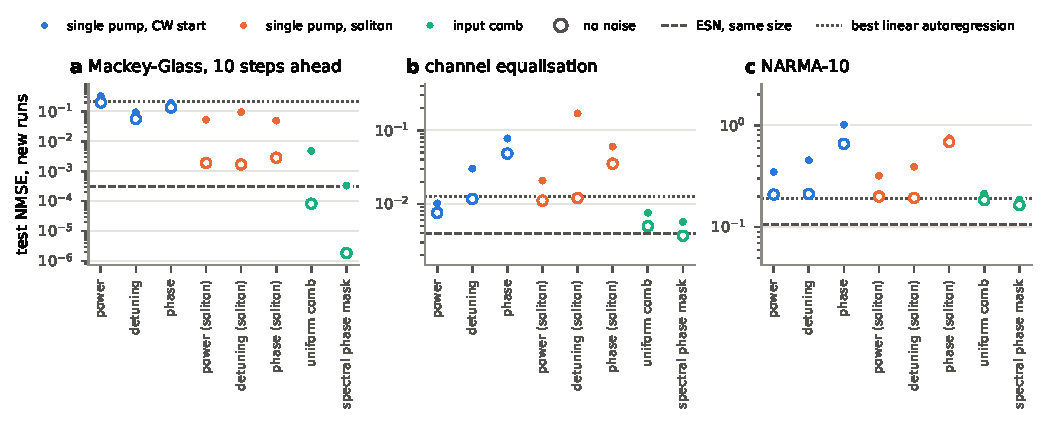
\includegraphics[width=\linewidth]{fig4_encodings}
\caption{Test error of the eight encodings on the three tasks under realistic noise (the ``realistic noise'' columns of
Table~\ref{tab:encodings}; new runs, geometric mean over three series).
Blue: single-pump encodings starting from an empty cavity; orange: single-pump encodings starting from a single soliton; green:
input combs (uniform modulation and spectral-phase mask). Dashed: ESN with the same readout dimension (input noise
$3\times10^{-3}$); dotted: best linear autoregression.
(a) Mackey--Glass, ten steps ahead; (b) nonlinear channel equalisation; (c) NARMA-10.}
\label{fig:encodings}
\end{figure}

\subsection{Mackey--Glass prediction}

The spectral-phase mask has its largest advantage on Mackey--Glass. Without noise its test error is $1.8\times10^{-6}$, about 45
times better than the uniformly modulated comb ($8.2\times10^{-5}$), about 900 times better than the best single-pump encoding
(detuning, soliton start, $1.7\times10^{-3}$), and four to five orders of magnitude better than single-pump encodings starting
from an empty cavity. Under realistic noise every encoding degrades but the order stays: the mask reaches $3.3\times10^{-4}$, the
uniform comb $4.8\times10^{-3}$ (about 15 times worse) and the best single-pump encoding $5.0\times10^{-2}$ (about 150 times
worse).

The ESN with the same readout dimension reaches $2.4\times10^{-5}$ without noise, 13 times worse than the mask; under realistic
noise it reaches $3.2\times10^{-4}$, on par with the mask. The latter comparison depends on the input noise given to the ESN
($3\times10^{-3}$ here) and on using a single random reservoir: with several reservoirs the ESN reaches $1.9\times10^{-4}$, and with
input noise $10^{-3}$ it reaches $5.3\times10^{-5}$. Section~\ref{sec:software} is devoted to this comparison; this section only
compares optical encodings, which share one noise model and are not affected by the convention.

\subsection{The advantage does not come from one lucky operating point}

The best result of an encoding might just be one particularly good draw out of 256. Figure~\ref{fig:distributions} shows the error
distribution over all random operating points of each encoding (Mackey--Glass under realistic noise, 768 points over three series).
The whole distribution of the mask is shifted: its median, $4.3\times10^{-2}$, is already better than the best 10\% of every
single-pump encoding ($0.14$ to $0.38$), and its best 10\% lie below $1.9\times10^{-3}$, more than an order of magnitude better than
the best 10\% of the uniform comb ($2.5\times10^{-2}$). The advantage is thus a property of this class of input, not of a
particular parameter combination.

\begin{figure}[htbp]
\centering
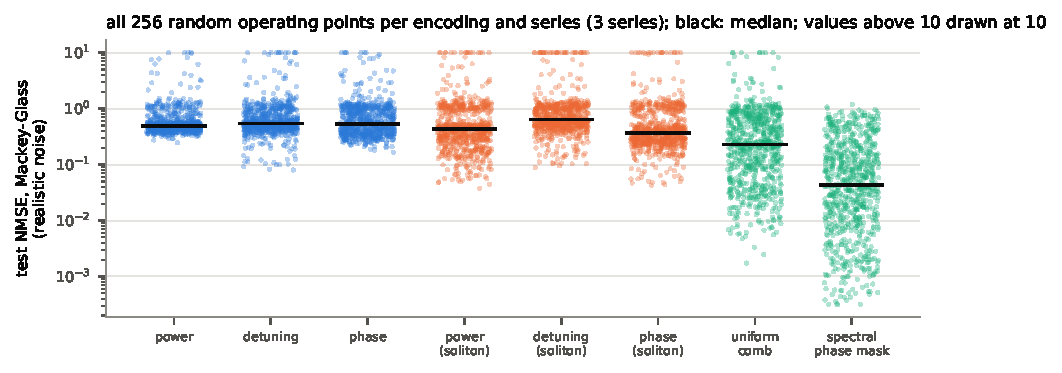
\includegraphics[width=\linewidth]{fig5_distributions}
\caption{Distribution of the Mackey--Glass test error under realistic noise: 256 random operating points per encoding and series
(768 points over three series, one pair of runs per point); black bars are medians, values above 10 are drawn at 10. Colours as in
Fig.~\ref{fig:encodings}.}
\label{fig:distributions}
\end{figure}

\subsection{Channel equalisation}

The differences are much smaller on channel equalisation. The mask is still the best optical encoding, $3.7\times10^{-3}$ without
noise and $5.7\times10^{-3}$ with realistic noise: about 1.3 times better than the uniform comb, about 2 times better than the best
single-pump encoding (power) and 2 to 3 times better than linear autoregression ($1.1\times10^{-2}$ and $1.3\times10^{-2}$).
Without noise the mask ties with the ESN ($3.8\times10^{-3}$); with realistic noise the ESN reaches $4.0\times10^{-3}$, about 1.4
times better than the mask. The error of this task comes mostly from the channel's own noise; Section~\ref{sec:software} shows that
removing the ESN's input noise entirely improves it by only about 7\%.
In symbol error rate (six new runs of 5000 test symbols per series, 90\,000 symbols over three series) the mask reaches
$1.9\times10^{-4}$ (17 errors), the uniform comb $1.0\times10^{-4}$ (9), the power encoding $3.9\times10^{-4}$ (35) and the ESN
$1.1\times10^{-5}$ (1). The mask and the uniform comb cannot be separated by this statistic; all comb encodings and the ESN are far
below the common hard-decision FEC threshold of $3.8\times10^{-3}$.

\subsection{NARMA-10: where a single ring does not work}

NARMA-10 needs a memory of about ten symbols, whereas the resonator's own memory is its photon lifetime, a few symbols at most.
With a single resonator the mask ($0.16$ without noise, $0.19$ with realistic noise) only ties with linear autoregression ($0.19$),
slightly better than the uniform comb and the single-pump encodings but 1.5 to 1.8 times worse than the ESN ($0.11$). We report this
as a negative case. Memory can be added from outside: with a delayed copy of the signal on the input lines (an input delay line)
and several rings with different masks read out together, NARMA-10 drops to $0.011$, on par with a 100-node ESN with the same delay
line ($0.010$; Section~\ref{sec:memory}).

\subsection{What matters is the randomness of the line phases}\label{sec:ablation}

To find out which part of the mask matters, we compared simplified masks over the same operating-point ranges (realistic noise,
the protocol of Table~\ref{tab:encodings}, 128 points each; Appendix~\ref{app:ablation}). On Mackey--Glass:
\begin{itemize}
\item random phases with equal line amplitudes: $2.4\times10^{-4}$, as good as or slightly better than the full mask
      ($3.8\times10^{-4}$ in this set of runs);
\item random amplitudes with all lines in phase: $1.3\times10^{-3}$, 3 to 6 times worse;
\item a random static spectrum with one common modulation ($w_\mu\propto b_\mu$): $6.5\times10^{-4}$;
\item equal amplitudes and phases (uniform modulation): $5.0\times10^{-3}$.
\end{itemize}
Channel equalisation gives the same order with smaller differences (phases only $5.0\times10^{-3}$, full mask $5.4\times10^{-3}$,
amplitudes only $5.8\times10^{-3}$, uniform $7.3\times10^{-3}$).
The number of input lines matters too: on Mackey--Glass 4, 8, 16, 32 and 64 lines give $1.9\times10^{-3}$, $1.4\times10^{-3}$,
$3.8\times10^{-4}$, $2.4\times10^{-4}$ and $2.1\times10^{-4}$, with little further gain beyond 32; on channel equalisation 32 lines
are best ($4.0\times10^{-3}$) and 64 are worse ($5.6\times10^{-3}$).

This gives the first design rule: \emph{what matters is the randomness of the line phases, not independent amplitude modulation of
each line}. No per-line modulators are needed; one modulator and two phase-only spectral shapers suffice.
We do not yet have a complete explanation of why phases matter more than amplitudes. An intuitive guess is that random phases make
the four-wave-mixing paths from different input lines into a given output line interfere differently, so that the line features are
less correlated with each other. At the linear level this guess fails. At the operating point chosen for each variant (no noise,
Mackey--Glass) we computed the correlation matrix of the 31 line features: the effective rank (participation ratio, the squared sum
of the eigenvalues divided by the sum of their squares) is $2.2$, $2.3$, $2.4$, $2.2$ and $2.0$ for the uniform comb, the random
spectrum with common modulation, amplitudes only, phases only and the full mask, and the mean absolute correlation is $0.58$,
$0.58$, $0.57$, $0.60$ and $0.65$. The variants are nearly identical, and the full mask even has the lowest linear diversity. The
benefit of the mask therefore does not lie in linear decorrelation of the instantaneous features; more likely the features are
different higher-order nonlinear functions of the input history. Testing this needs a decomposition such as the information
processing capacity and is left for future work.
